\documentclass[12pt]{article}

\usepackage{graphicx}
\usepackage[a4paper,left=2.6cm, right=2.9cm,top=3cm, bottom=3.5cm]{geometry}

\begin{document}
\section*{Abgabe OMP Blatt 01}
Weerts, Steffen, steffen.weerts@uni-oldenburg.de. Gruppenname: 17
\subsection*{Aufgabe 1}
\begin{enumerate}
	\item[(a)] UML-Klassendiagramm:
	\begin{center}
		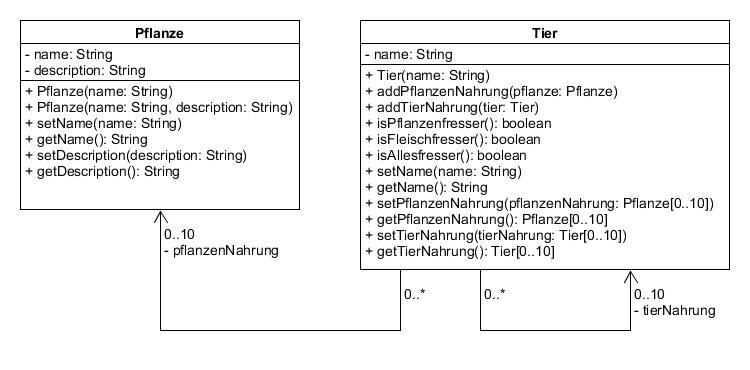
\includegraphics[scale=0.5]{OMP_Blatt01_Weerts_Klassendiagramm_a.jpg}
	\end{center}
	
	\item[(b)] Java-Implementierung der Klassen Pflanze und Tier: \\
	(Der Quellcode befindet sich auch als .java Datei im Anhang)
	\begin{center}
		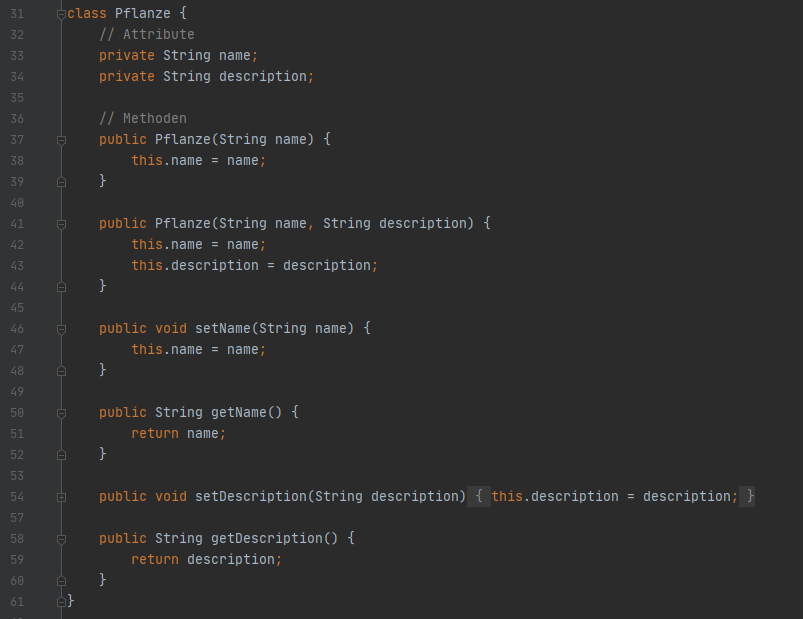
\includegraphics[scale=.65]{Quellcode_Pflanze.png}
		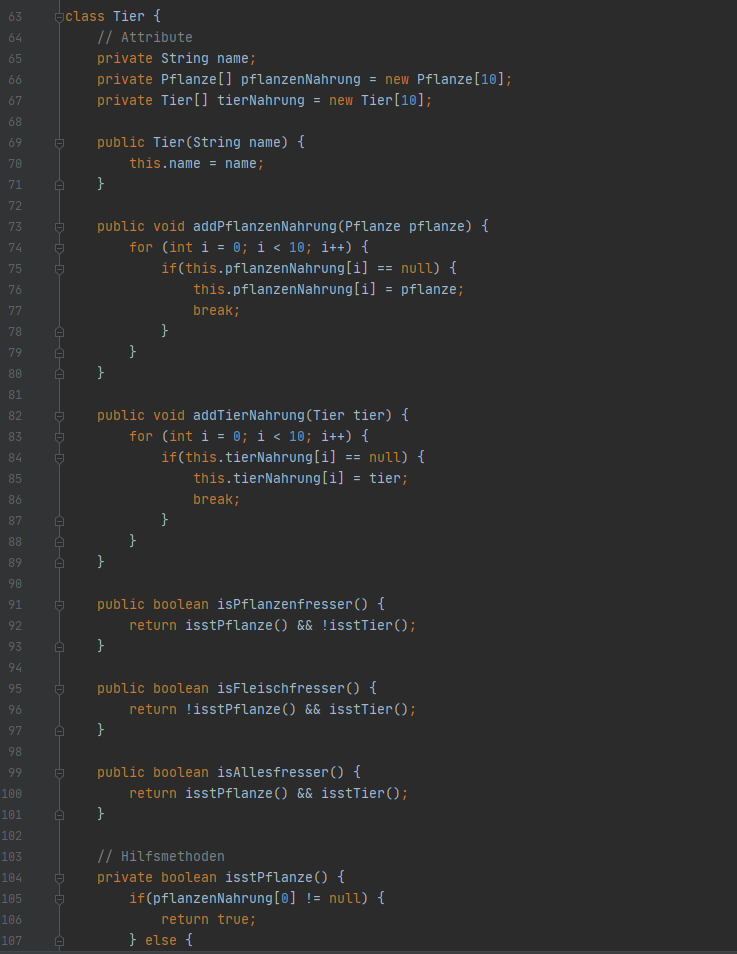
\includegraphics[scale=.7]{Quellcode_Tier_1.png}
		(Fortsetzung auf nächster Seite)
		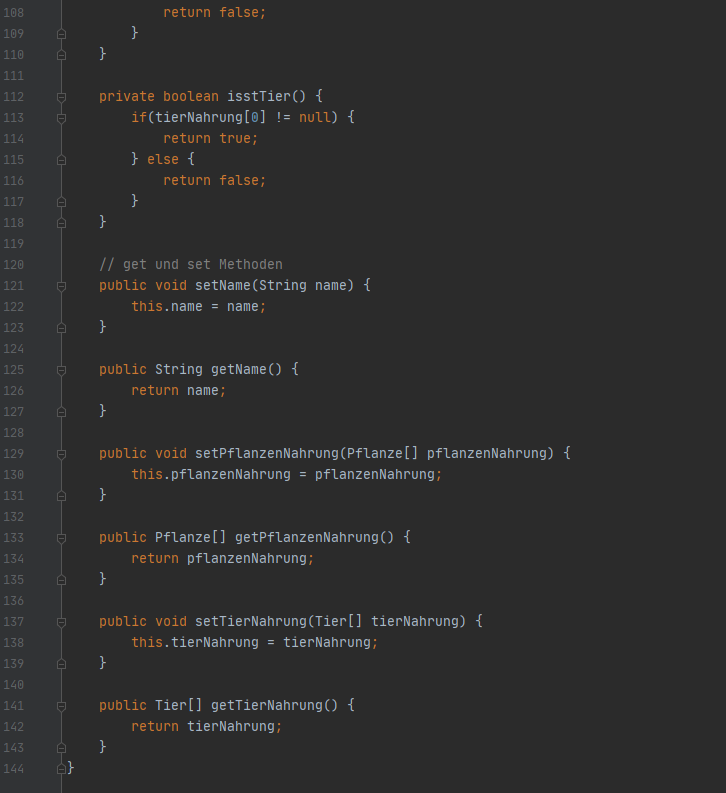
\includegraphics[scale=.7]{Quellcode_Tier_2.png}
	\end{center}
	
	\item[(c)] UML-Klassendiagramm
	\begin{center}
		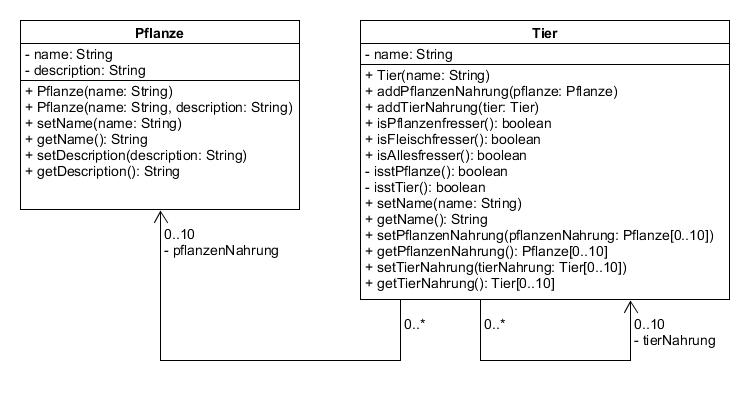
\includegraphics[scale=.5]{OMP_Blatt01_Weerts_Klassendiagramm.jpg}
	\end{center}
	
	\item[(d)] Java-Implementierung des Programms BioTest, welches die obigen Klassen verwendet: \\
	(Der Quellcode befindet sich auch als .java Datei im Anhang)
	\begin{center}
		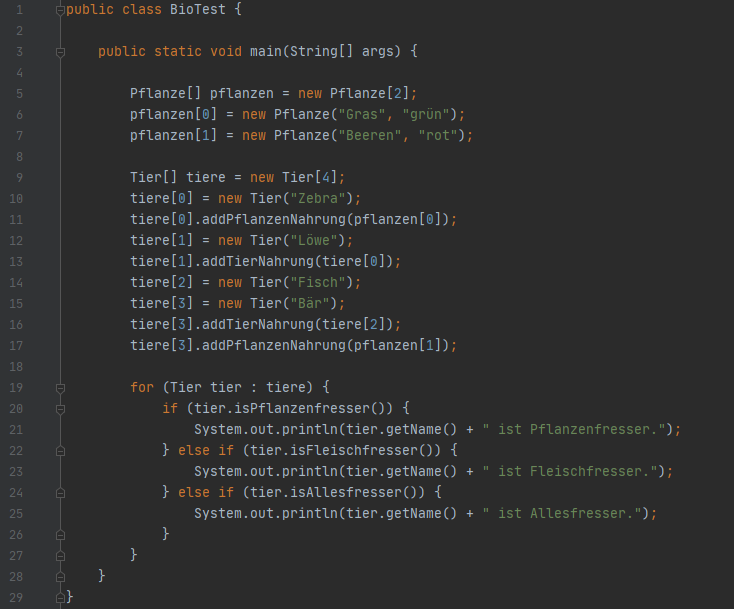
\includegraphics[scale=.7]{Quellcode_BioTest.png}
	\end{center}
	
	\item[(e)] UML-Objektdiagramm am Ende der Ausführung des Programms:
	\begin{center}
		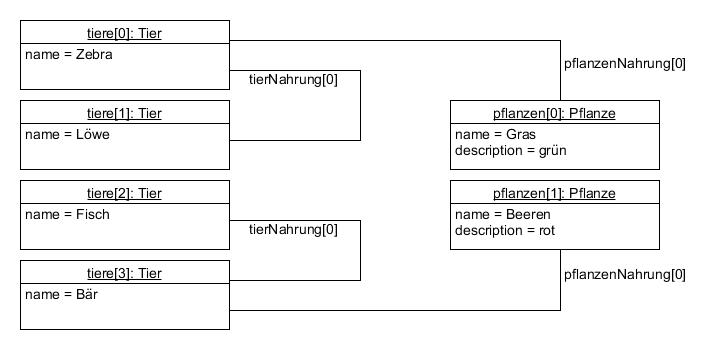
\includegraphics[scale=.5]{OMP_Blatt01_Weerts_Objektdiagramm.jpg}
	\end{center}
\end{enumerate}
\end{document}